\documentclass[letterpaper,12pt]{article}
\usepackage{tabularx} % extra features for tabular environment
\usepackage{amsmath}  % improve math presentation
\usepackage{graphicx} % takes care of graphic including machinery
\usepackage[margin=1in,letterpaper]{geometry} % this shaves off default margins which are too big
\usepackage{cite}
\usepackage[final]{hyperref} % adds hyper links inside the generated pdf file
\hypersetup{
	colorlinks=true,       % false: boxed links; true: colored links
	linkcolor=blue,        % color of internal links
	citecolor=blue,        % color of links to bibliography
	filecolor=magenta,     % color of file links
	urlcolor=blue         
}

\begin{document}

\title{Title of the experiment}
\author{Y. O. Urname, partners:  P. A. RtnerA, and P. A. RtnerB}
\date{\today}
\maketitle

\begin{abstract}
In this experiment we studied a very important physical effect by measuring the
dependence of a quantity $V$ of the quantity $X$ for two different sample
temperatures.  Our experimental measurements confirmed the quadratic dependence
$V = kX^2$ predicted by Someone's first law. The value of the mystery parameter
$k = 15.4\pm 0.5$~s was extracted from the fit. We found that this value is
20\% below theoretically predicted $k_{theory}=17.34$~s. We attribute this
discrepancy to low efficiency of our $V$-detector.
\end{abstract}


% Everything behind the % symblol will be invisible in the final document
% i.e. it is a comment for the writer not a reader


\section{Theory overview}
Here give a brief summary of the physical effect of interest and provide
necessary equations. Here is how you insert an equation. According to
references~\cite{melissinos, Cyr, Wiki} the dependence of interest is given
by
\begin{equation} \label{eq:aperp}
u(\lambda,T)=\frac{8\pi hc\lambda^{-5}}{e^{hc/\lambda kT}-1},
\end{equation}
where T is temperature in Kelvin, c is the speed of light, etc. Don't forget to
explain what each variable in the equation means, when you introduce it for the
first time!


% notice how text below references equations, figures, and tables via
% \label and \ref commands.
% DO NOT DO something like: see Eq. 1 and Fig. 1
% instead DO: see Eq.~\ref{eq:aperp} and Fig.~\ref{fig:samplesetup} 
% Note the ~ symbol it means non breakable space.
% Same goes for tables.
% One day you will write a thesis with a lot figures and equation, and you
% will not want to track the numbering manually. This is what for computers
% are.


\section{Experimental setup and procedures}

{\bf Note:} LaTeX will put figures and tables at the locations
where it thinks it is the best. Do not fight it,
unless you really need it.

Give a schematic of the experimental setup(s) used in the experiment (see
figure~\ref{fig:samplesetup}). Give the description of  abbreviations
either in the figure caption or in the text. Write a description of what is
going on. 

\begin{figure}[ht] 
        % read manual to see what [ht] means and for other possible options
        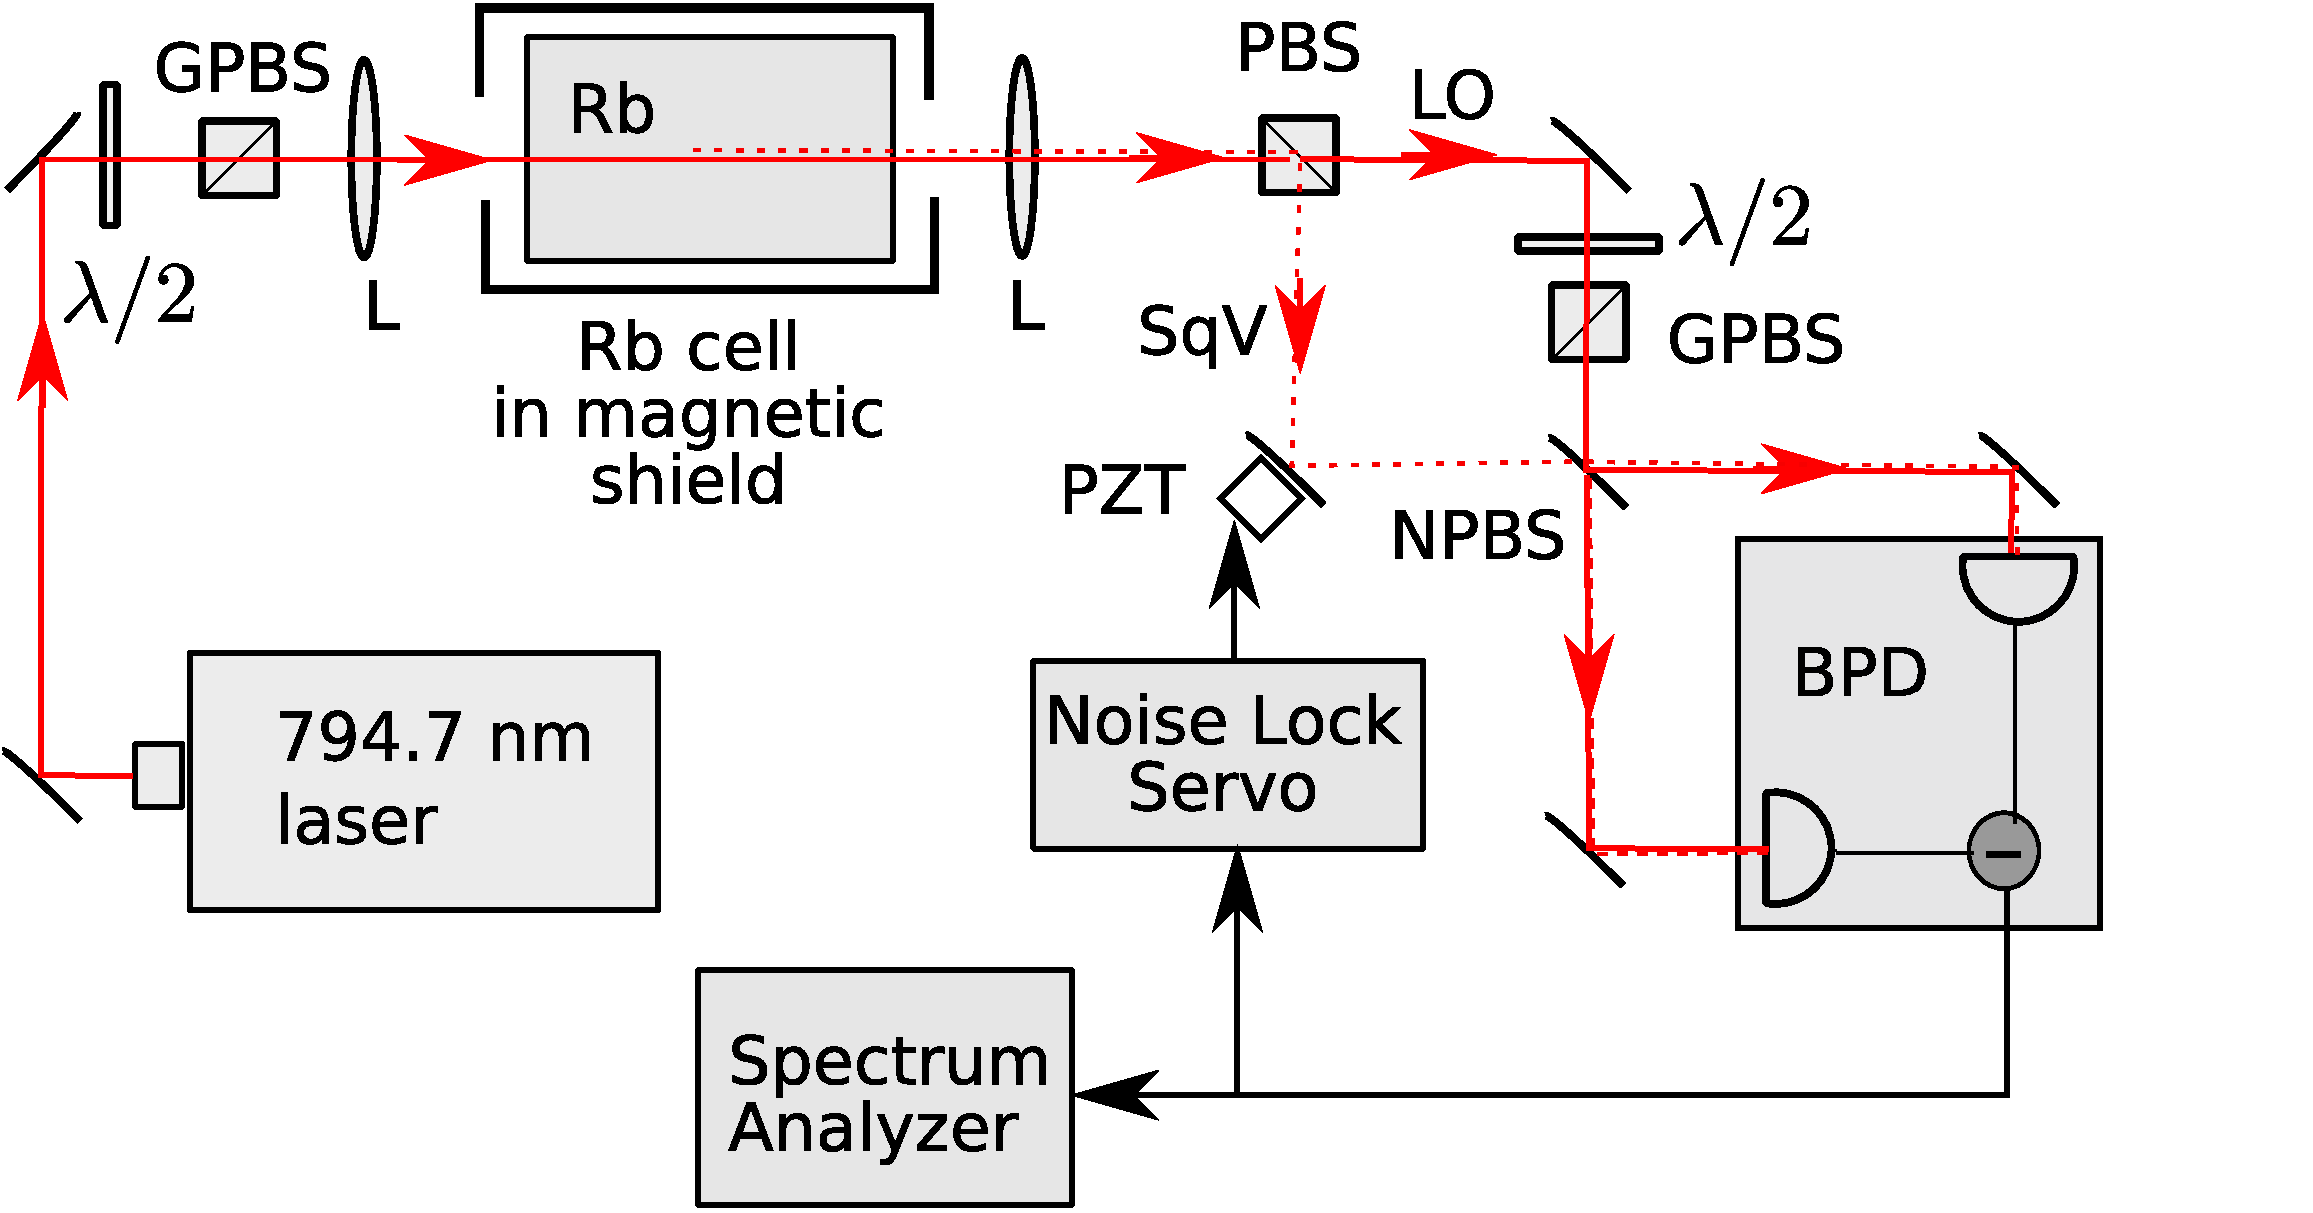
\includegraphics[width=1.0\columnwidth]{sr_setup}
        % note that in above ___________________^^^^^^^^^figure file name
        % the file extension is missing. LaTeX is smart enough to find
        % apropriate one (i.e. pdf, png, etc.)
        % You can add this extention yourself as it seen below
        % both notations are correct but above has more flexibility
        %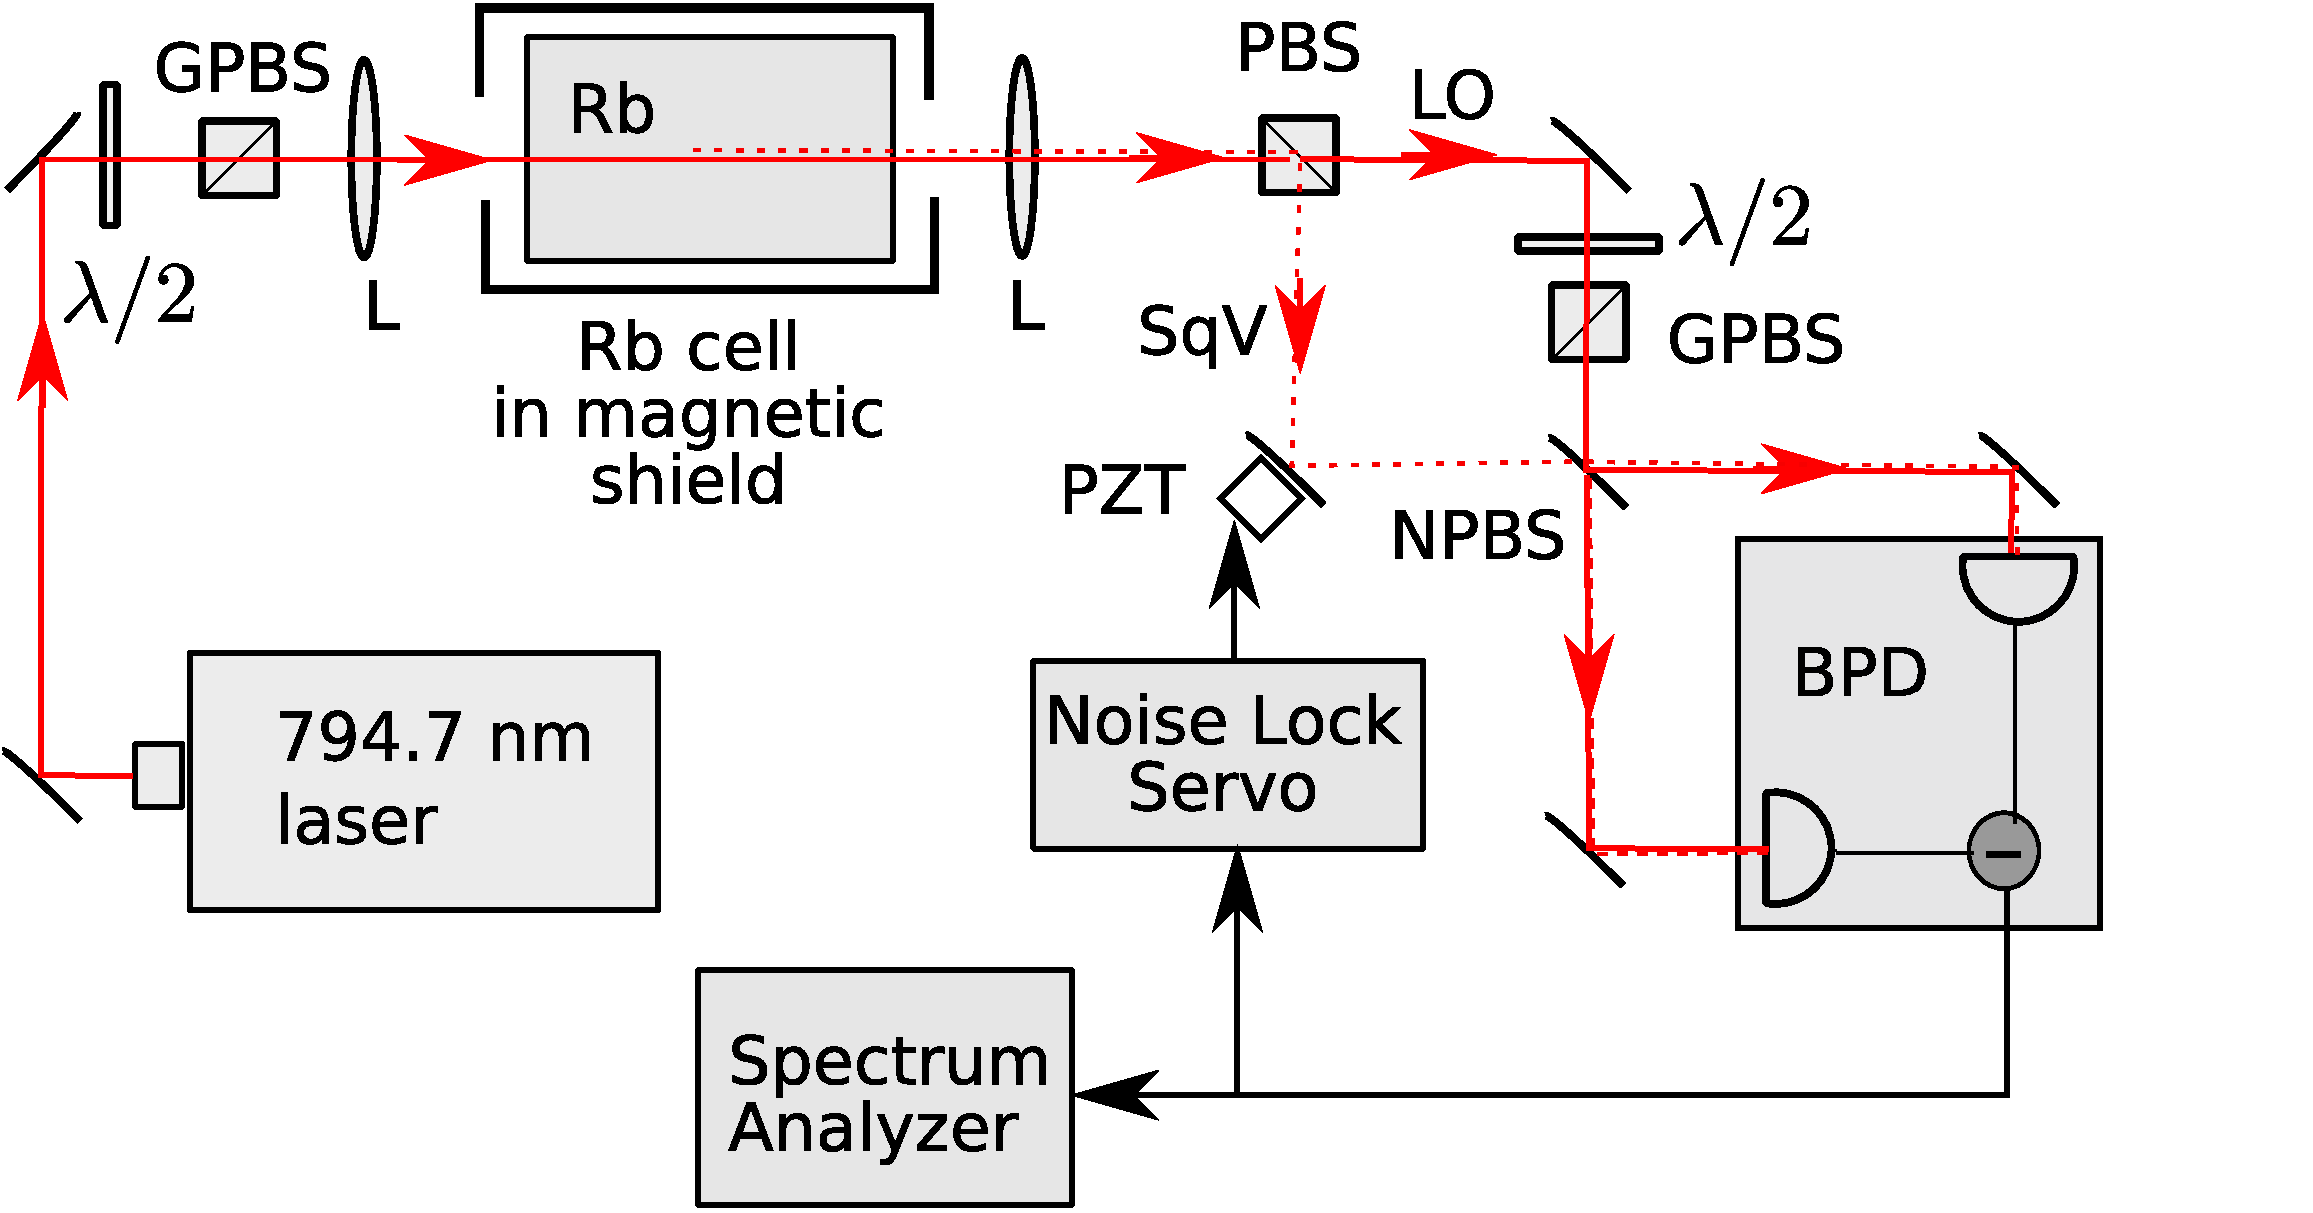
\includegraphics[width=1.0\columnwidth]{sr_setup.pdf}
        \caption{
                \label{fig:samplesetup} % spaces are big no-no withing labels
                % things like fig: are optional in the label but it helps
                % to orient yourself when you have multiple figures,
                % equations and tables
                {\bf  Every figure MUST have a caption.}
                Experimental setup. 
                SMPM fiber depicts single-mode polarization-maintaining fiber,
                $\lambda/2$ is half-wave plate,
                PhR is phase-retarding wave plate,
                PBS is polarizing beam splitter,
                GP is Glan-laser polarizer,
                and BPD is balanced photodetector.
        }
\end{figure}

Don't forget to list all important steps in your experimental procedure!

Use active voice either in past or present through all the report and be
consistent with it:
The laser light comes  from to ... and eventually arrived to the
balanced photodiode as seen in the figure~\ref{fig:samplesetup}.

Sentences in the past voice while correct are generally considered hard to read
in large numbers. The laser light was directed to ..., wave plates were set
to ... etc.


\section{Experimental data and the data analysis}

In this section you will need to show your experimental results. Use tables and
graphs when it is possible. Table~\ref{tbl:bins} is an example.

\begin{table}[ht]
\begin{center}
\caption{Every table needs a caption}
\label{tbl:bins} % spaces are big no-no withing labels
\begin{tabular}{|ccccccc|} \hline
\multicolumn{1}{|c}{Polarization} & \multicolumn{1}{c}{Target} &
\multicolumn{1}{c}{Bin} & \multicolumn{1}{c}{$<x>$} &
\multicolumn{1}{c}{$<Q^2>$} & \multicolumn{1}{c}{$A_{\perp}^{meas}$} &
\multicolumn{1}{c|}{$\Delta A_{\perp}$} \\
\hline
$-$ & LiD     & 1 &   0.0233323 &   0.8429978  &   0.0044151 &   0.0030871 \\
    &         & 2 &   0.0638046 &   1.5017358  &   0.0021633 &   0.0021343 \\
    &         & 3 &   0.1892825 &   3.1877837  &   0.0006640 &   0.0022467 \\
    &         & 4 &   0.4766562 &   7.1827556  &  -0.0197585 &   0.0085528 \\
    & NH$_3$  & 1 &   0.0232572 &   0.8454089  &   0.0003600 &   0.0018642 \\
    &         & 2 &   0.0633156 &   1.4870013  &   0.0023831 &   0.0013287 \\
    &         & 3 &   0.1923955 &   3.1753302  &  -0.0024246 &   0.0013771 \\
    &         & 4 &   0.4830315 &   7.3245904  &  -0.0284834 &   0.0047061 \\
$+$ & LiD     & 1 &   0.0233503 &   0.8340932  &  -0.0086018 &   0.0031121 \\
    &         & 2 &   0.0638688 &   1.4785886  &  -0.0018465 &   0.0021452 \\
    &         & 3 &   0.1892192 &   3.1277721  &  -0.0017860 &   0.0022525 \\
    &         & 4 &   0.4778486 &   7.0313856  &  -0.0041773 &   0.0084659 \\
    & NH$_3$  & 1 &   0.0232964 &   0.8439092  &  -0.0022961 &   0.0018851 \\
    &         & 2 &   0.0633764 &   1.4814540  &   0.0021355 &   0.0013354 \\
    &         & 3 &   0.1924094 &   3.1580557  &  -0.0065302 &   0.0013775 \\
    &         & 4 &   0.4825868 &   7.3191291  &  -0.0290878 &   0.0047329 \\
\hline
\end{tabular}
\end{center}
\end{table}

\subsection{Error analysis}

Analysis of equation~\ref{eq:aperp} shows ...

Note: this section can be integrated with the previous one as long as you
address the issue. Here explain how you determine uncertainties for different
measured values. Suppose that in the experiment you make a series of
measurements of a resistance of the wire $R$ for different applied voltages
$V$, then you calculate the temperature from the resistance using a known
equation and make a plot  temperature vs. voltage squared. Again suppose that
this dependence is expected to be linear~\cite{Cyr}, and the proportionality coefficient
is extracted from the graph. Then what you need to explain is that for the
resistance and the voltage the uncertainties are instrumental (since each
measurements in done only once), and they are $\dots$. Then give an equation
for calculating the uncertainty of the temperature from the resistance
uncertainty. Finally explain how the uncertainty of the slop of the graph was
found (computer fitting, graphical method, \emph{etc}.)

If in the process of data analysis you found any noticeable systematic
error(s), you have to explain them in this section of the report.

It is also recommended to plot the data graphically to efficiently illustrate
any points of discussion. For example, it is easy to conclude that the
experiment and theory match each other rather well if you look at
Fig.~\ref{fig:samplesetup} and Fig.~\ref{fig:exp_plots}.

\begin{figure}[ht] 
        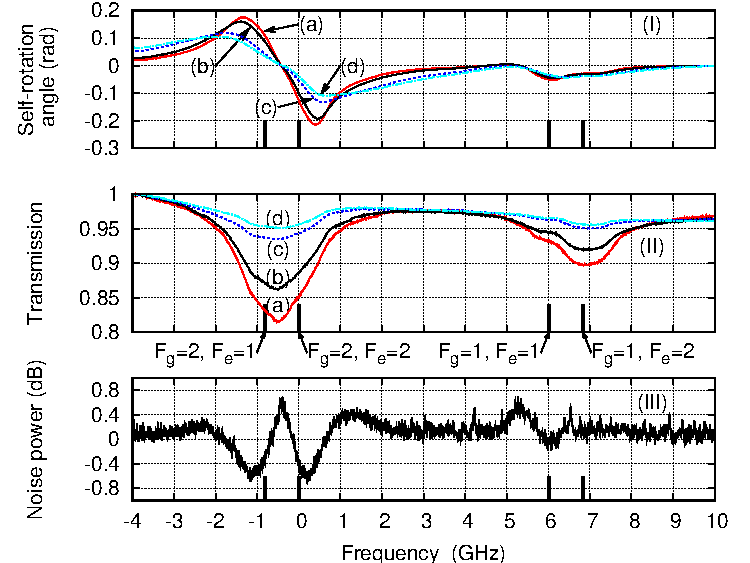
\includegraphics[width=0.5\columnwidth]{sr_squeezing_vs_detuning}
        % some figures do not need to be too wide
        \caption{
                \label{fig:exp_plots}  % spaces are big no-no withing labels
                % things like fig: are optional in the label but it helps
                % to orient yourself when you have multiple figures,
                % equations and tables
                {\bf Every figure MUST have a caption.}
                {\bf Every plot MUST have axes labeled.}
                The dependence of self rotation and squeezing on the laser
                detunings.
        }
\end{figure}


\section{Necessary remarks}

Context of this template is out of sync with figures, tables, references,
etc. It is just a template with examples how to use particular \LaTeX{}
features.

\section{Conclusions}
Here you briefly summarize your findings.

%++++++++++++++++++++++++++++++++++++++++

% References section will be created automatically 
% with inclusion of "thebibliography" environment
% as it shown below. See text starting with line
% \begin{thebibliography}{99}




% There is a fancier and in long run more convenient way to do bibliography 
% with automatic inclusion of references from the bibliography database
% file. See usage of "bibtex" if you are interested in it.
% http://www.bibtex.org/
% but for know we will go with hand formatted list.
% Note: with this approach it is YOUR responsibility to put them in order
% of appearance.
\begin{thebibliography}{99}


\bibitem{melissinos}
A.~C. Melissinos and J. Napolitano, \textit{Experiments in Modern Physics},
(Academic Press, New York, 2003).

\bibitem{Cyr}
N.\ Cyr, M.\ T$\hat{e}$tu, and M.\ Breton,
% "All-optical microwave frequency standard: a proposal,"
IEEE Trans.\ Instrum.\ Meas.\ \textbf{42}, 640 (1993).

\bibitem{Wiki} \emph{Expected value},  available at
\url{http://en.wikipedia.org/wiki/Expected_value}.

\end{thebibliography}


\end{document}
